\subsubsection{Characteristic faults}
\index{Source type!fault!characteristic}
\index{Characteristic fault|see{Source type}}

The charactercistic fault source is a particular typology of fault created
with the assumption that its ruptures will always cover the entire fault
surface.

In this case, the fault surface can be represented either as a
\gls{simplefaultsource} surface or as a \gls{complexfaultsource} surface or as
a combination of rectangular ruptures as represented in
Figure~\ref{fig:char_fault_source}.

\begin{figure}[!ht]
\centering
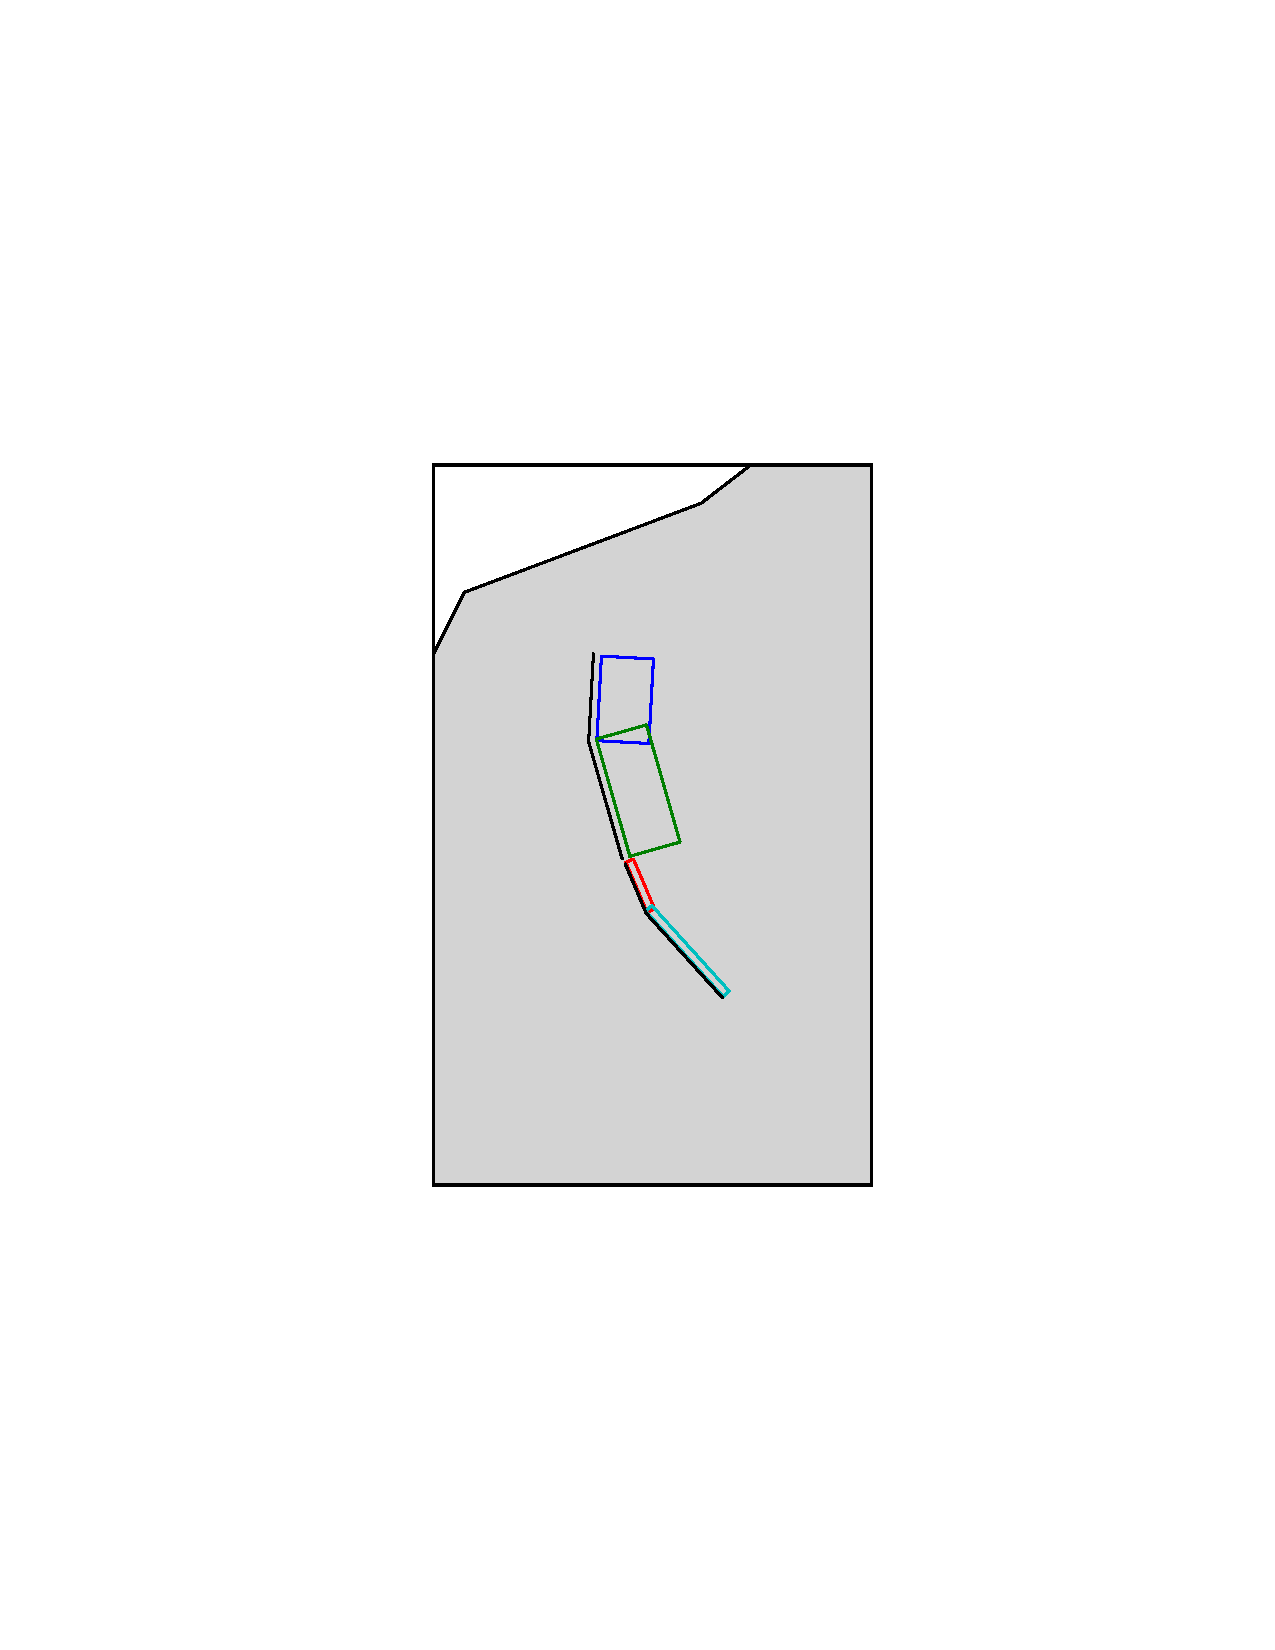
\includegraphics[width=15cm]{figures/hazard/multi_surface.pdf}
\caption{Geometry of a multi-segmented characteristic fault composed of four
         rectangular ruptures as modelled in OpenQuake.}
\label{fig:char_fault_source}
\end{figure}

\paragraph{Source data}

\begin{itemize}

    \item The characteristic rupture surface is defined through one of the
    following options:

        \begin{itemize}

            \item A list of rectangular ruptures

            \item A \gls{simplefaultsource} geometry

            \item A \gls{complexfaultsource} geometry

        \end{itemize}

    \item A \gls{frequencymagnitudedistribution}.

    \item Rake angle (specified following the Aki-Richards convention; see
          \citet{aki2002}).

    \item Upper and lower depth values limiting the seismogenic interval.

\end{itemize}
